\documentclass[12pt,a4paper]{article}
 \usepackage[italian]{babel}
 \usepackage[latin1]{inputenc}
 \usepackage{verbatim}
 \usepackage{amsmath}
 \usepackage{graphicx}
 \usepackage{url}
 \usepackage{geometry}
 \usepackage{color}
 \usepackage{subfigure}
 \geometry{a4paper,top=3cm,bottom=3cm,left=2cm,right=2cm,heightrounded,bindingoffset=1cm}
 
 \begin{document}
 	\title{Matematical model of a three mass and three damped spring system} \author{Matteo Bolognese}
 	\date{23/11/2019}
 	\maketitle
 	
 \section{Introduction}
	A teoretical model is useful to validate the measurement of the physical system, and to estimate the physical quantities. The phisical configuration is represented in \figurename~\ref{fig:Phisical-configuration} and include a metallic plate, the tample and the base.
	
	\begin{figure}
		\centering
		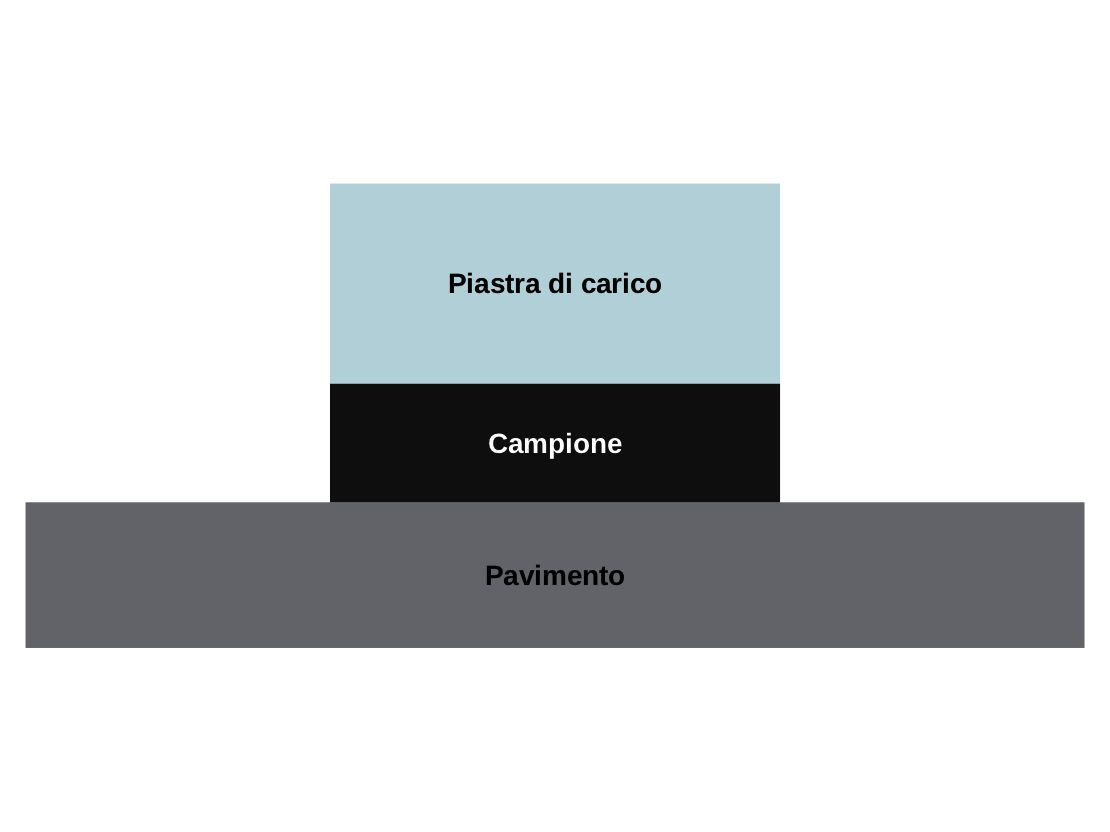
\includegraphics[width=13cm]{Phisical-system}
		\caption{Phisical configuration.}
		\label{fig:Phisical-configuration}
	\end{figure}
 	
 \section{Three mass - three damped spring sistem}
 	The easiest way to represent the system in \figurename~\ref{fig:Phisical-configuration} is represented in \figurename~\ref{fig:model} where index $1$ refers to the plate, index $2$ refers to the sample, and index $3$ refers to the floor.
 	
 	\begin{figure}
 		\centering
 		%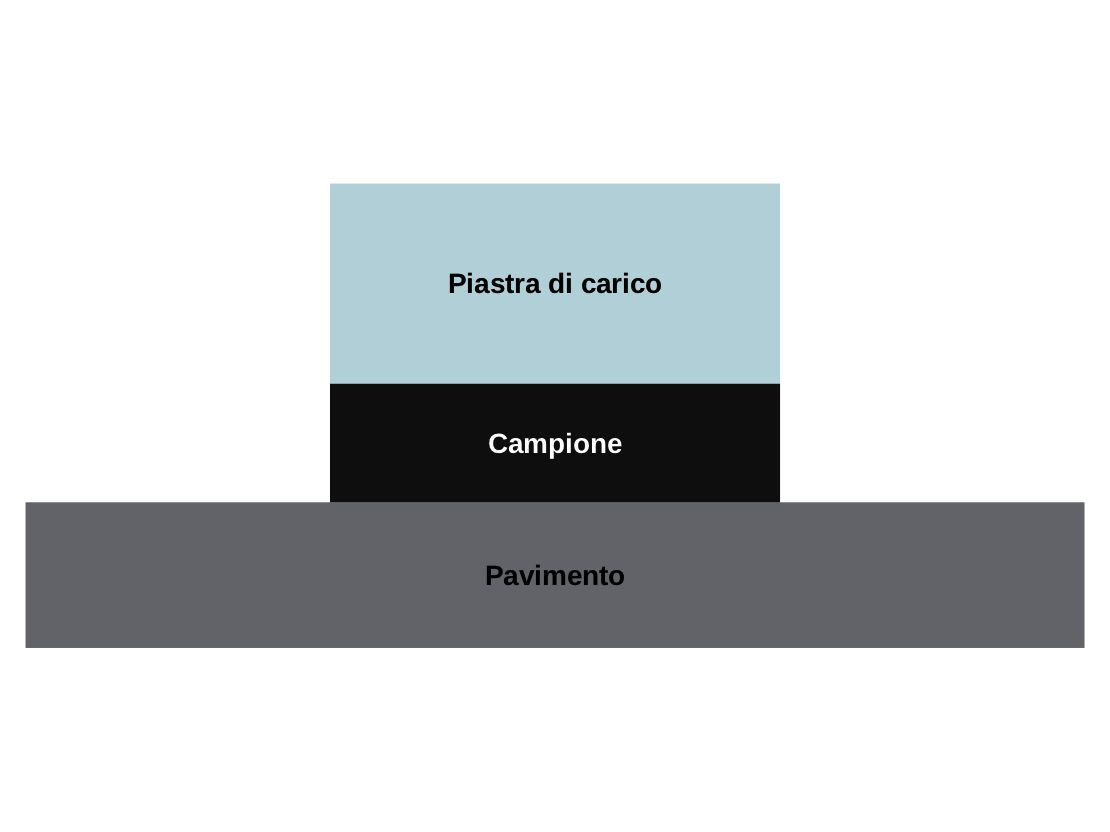
\includegraphics[width=13cm]{Phisical-system}
 		\caption{Theoretical model.}
 		\label{fig:model}
 	\end{figure}
 
 
 
 
 \end{document}